\documentclass{article}
\usepackage[francais]{babel}
\usepackage[utf8]{inputenc} % Required for including letters with accents
\usepackage[T1]{fontenc} % Use 8-bit encoding that has 256 glyphs
\usepackage{pythontex}
\usepackage{amsthm}
\usepackage{amsmath}
\usepackage{amssymb}
\usepackage{mathrsfs}
\usepackage{graphicx}
\usepackage{geometry}
\usepackage{stmaryrd}
\usepackage{tikz}
\usetikzlibrary{patterns}
%\usetikzlibrary{intersections}
\usetikzlibrary{calc} 
%\usepackage{tkz-tab}
\usepackage{stmaryrd}
%\usepackage{tikz}
%\usetikzlibrary{tikzmark}
\usepackage{empheq}
\usepackage{longtable}
\usepackage{booktabs} 
\usepackage{array}
\usepackage{pstricks}
\usepackage{pst-3dplot}
\usepackage{pst-tree}
\usepackage{pstricks-add}
\usepackage{upgreek}
%\usepackage{epstopdf}
\usepackage{eolgrab}
\usepackage{chngpage}
 \usepackage{calrsfs}
 % Appel du package pythontex 
\usepackage{pythontex}
 \usepackage{enumitem}
\usetikzlibrary{decorations.pathmorphing}
\def \de {{\rm d}}
\def \ch {{\rm ch}}
\def \sh {{\rm sh}}
\def \th {{\rm th}}

\usepackage{color}
%\usepackage{xcolor}
%\usepackage{textcomp}
\newcommand{\mybox}[1]{\fbox{$\displaystyle#1$}}
\newcommand{\myredbox}[1]{\fcolorbox{red}{white}{$\displaystyle#1$}}
\newcommand{\mydoublebox}[1]{\fbox{\fbox{$\displaystyle#1$}}}
\newcommand{\myreddoublebox}[1]{\fcolorbox{red}{white}{\fcolorbox{red}{white}{$\displaystyle#1$}}}

\definecolor{purple2}{RGB}{153,0,153} % there's actually no standard purple
\definecolor{green2}{RGB}{0,153,0} % a darker green
\usepackage{xcolor}
\usepackage{listings}

\lstdefinestyle{Python}{
    language        = Python,
    basicstyle      = \ttfamily,
    keywordstyle    = \color{blue},
    keywordstyle    = [2] \color{teal}, % just to check that it works
    stringstyle     = \color{violet},
    commentstyle    = \color{red}\ttfamily
}

\usepackage{amsmath} 
\renewcommand{\overrightarrow}[1]{\vbox{\halign{##\cr 
  \tiny\rightarrowfill\cr\noalign{\nointerlineskip\vskip1pt} 
  $#1\mskip2mu$\cr}}}

\newcommand{\Coord}[3]{% 
  \ensuremath{\overrightarrow{#1}\, 
    \begin{pmatrix} 
      #2\\ 
      #3 
    \end{pmatrix}}}

\newcommand{\norme}[1]{\left\lVert\overrightarrow{#1}\right\rVert}
\newcommand{\vecteur}[1]{\overrightarrow{#1}}
  \title{Enseignement de la Méthode des Éléments Finis en tronc commun à l'ESTP}
  %\author{ \textsc{Ibrahim ALAME}}
%\date{23/04/2021}
  \begin{document}
  \lstset{
    frame       = single,
    numbers     = left,
    showspaces  = false,
    showstringspaces    = false,
    captionpos  = t,
    caption     = \lstname
}
\maketitle
\subsubsection*{Outils d'analyse fonctionnelle }
\begin{itemize}[label=\textbullet, font=\small \color{blue}]
\item \underline{Rappels sur les distributions}
\item \underline{Espaces de Sobolev}
\[H^1(\Omega)=\{v\in L^2(\Omega), \frac{\partial v}{\partial x_i} \in L^2(\Omega)\}\]
$H^1(\Omega)$ est un espace de Hilbert. Plus généralement $H^m(\Omega)=\{v\in L^2(\Omega), \partial^\alpha v\in L^2(\Omega), |\alpha|\leq m\}$.
 \item \underline{Théorème de trace} , \[H_0^1(\Omega)=\{v\in H^1(\Omega), v_{/\Gamma}=0\}\]
\end{itemize}
\subsubsection*{Formulation variationnelle}
\begin{itemize}[label=\textbullet, font=\small \color{blue}]
\item \underline{Formule de Green:}
\[-\int_\Omega \Delta u\cdot v \; \de x = \int_\Omega \nabla u\cdot \nabla v \; \de x-\int_\Gamma  \frac{\partial v}{\partial \vec n} \cdot v \; \de \sigma\]
\item \underline{Problème aux limites elliptiques}
\begin{description}%[font=\small \color{red}]
\item [{\it Problème de Dirichlet:}]
\[\left\{\begin{array}{rl}
-\Delta u = f & \mbox{ dans }\Omega \\
u=0 & \mbox{ sur }\Gamma 
\end{array}\right.  \Longleftrightarrow \forall \varphi\in {\cal D}(\Omega),\; \int_\Omega \nabla u\cdot \nabla \varphi \; \de x=\int_\Omega f\,\varphi \; \de x\]
\item[{\it Problème de Neumann:}]
\[\left\{\begin{array}{rl}
-\Delta u + u= f & \mbox{ dans }\Omega \\
\frac{\partial v}{\partial \vec n} =0 & \mbox{ sur }\Gamma 
\end{array}\right.  \Longleftrightarrow \forall \varphi\in {\cal D}(\Omega),\; \int_\Omega \nabla u\cdot \nabla \varphi \; \de x + \int_\Omega u\cdot  \varphi \; \de x =\int_\Omega f\,\varphi \; \de x\]
\end{description}

\item \underline{Problèmes variationnels abstraits}
Trouver $u\in V$ tel que
\[\myredbox{\forall v\in V\quad a(u,v)=\ell(v)}\]
$\Longleftrightarrow$ Trouver  $u\in V$ tel que $\myredbox{J(u)=\min_{v\in V}J(v)}$ où $J(v)=\frac 12 a(v,v)-\ell(v)$.
\item \underline{Théorème de Lax-Milgram}
\item \underline{Système de l'élasticité}

\hfill $\left\{\begin{array}{rl}
\mbox{div}\,\sigma(u) + f= 0 & \mbox{ dans }\Omega \\
u=0 & \mbox{ sur }\Gamma_0 \\
\sigma(u)\vec n=g & \mbox{ sur }\Gamma_1 
\end{array}\right. $\hfill \includegraphics[scale=0.5]{elasticite2.png} 

où
\[\sigma_{ij}(v)=\lambda\left(\sum_{k=1}^n\varepsilon_{kk}\right)\delta_{ij}+2\mu\varepsilon_{ij}(v) \mbox{ et } \varepsilon_{ij}(v)=\frac 12\left(\frac{\partial v_i}{\partial x_j}+\frac{\partial v_j}{\partial x_i}\right)\]
La formulation variationnelle: Trouver $u\in V$ tel que $\forall v\in V\quad a(u,v)=\ell(v)$ où
\[a(u,v)=\sum_{i,j=1}^n\int_\Omega \sigma_{ij}(u)\varepsilon_{ij}(v)\,\de x\mbox{ et }\ell(v)=\sum_{i=1}^n\int_\Omega f_{i}\,v_i \,\de x + \int_{\Gamma_1} g_{i}\,v_i \,\de \sigma\]
Cas particuliers
\begin{description}
\item[Barres]: Trouver $u\in V=H^1(0,L)$ tel que: $\forall v\in V$ $a(u,v)=\ell(v)$, où
\[a(u,v)=\int_0^L ES u'v'\,\de x,\quad \mbox{ et } \quad \ell(v)=f_Lv(L)-f_0v(0)\]

\newcommand{\appui}[3]%
{\fill[fill=gray]   (#1,#2) -- (#1-#3*0.8,#2+#3*0.5)--(#1-#3*0.8,#2-#3*0.5)--cycle;
\fill[fill=gray] [pattern=north east lines]
     (#1-#3*0.8,#2+#3*0.5)
     --(#1-#3*0.8,#2-#3*0.5)
     -- (#1-#3*0.8-#3*0.5,#2-#3*0.5)
     -- (#1-#3*0.8-#3*0.5,#2+#3*0.5)
     -- cycle;

}
\begin{center}
\begin{tikzpicture}[scale=1]
\appui{0}{0}{.3};
\appui{0}{-2}{.3};
\draw[double distance = 1pt] (0,0) - - (2,0);
\draw[double distance = 1pt] (2,0) - - (4,0);
\draw[double distance = 1pt] (4,0) - - (6,0);
\draw[double distance = 1pt] (6,0) - - (4,-2);
\draw[double distance = 1pt] (4,-2) - - (2,-2);
\draw[double distance = 1pt] (2,-2) - - (0,-2);
\draw[double distance = 1pt] (4,0) - - (2,-2);
\draw[double distance = 1pt] (2,0) - - (0,-2);
\draw[double distance = 1pt] (2,0) - - (2,-2);
\draw[double distance = 1pt] (4,0) - - (4,-2);
\path[fill=black]  (0,0) circle (.75mm) [fill=gray];
\path[fill=black]  (2,0) circle (.75mm) [fill=gray];
\path[fill=black]  (4,0) circle (.75mm) [fill=gray];
\path[fill=black]  (6,0) circle (.75mm) [fill=gray];
\path[fill=black]  (4,-2) circle (.75mm) [fill=gray];
\path[fill=black]  (2,-2) circle (.75mm) [fill=gray];
\path[fill=black]  (0,-2) circle (.75mm) [fill=gray];

\draw[red,double distance = 1pt] (0.0,0.0) - - (2.0300000000000002,-0.07242640687119303);
\draw[red,double distance = 1pt] (2.0300000000000002,-0.07242640687119303) - - (4.045,-0.1898528137423861);
\draw[red,double distance = 1pt] (4.045,-0.1898528137423861) - - (6.045,-0.24985281374238621);
\draw[red,double distance = 1pt] (6.045,-0.24985281374238621) - - (3.985,-2.189852813742386);
\draw[red,double distance = 1pt] (3.985,-2.189852813742386) - - (1.9849999999999999,-2.087426406871193);
\draw[red,double distance = 1pt] (1.9849999999999999,-2.087426406871193) - - (0.0,-2.0);
\draw[red,double distance = 1pt] (4.045,-0.1898528137423861) - - (1.9849999999999999,-2.087426406871193);
\draw[red,double distance = 1pt] (2.0300000000000002,-0.07242640687119303) - - (0.0,-2.0);
\draw[red,double distance = 1pt] (2.0300000000000002,-0.07242640687119303) - - (1.9849999999999999,-2.087426406871193);
\draw[red,double distance = 1pt] (4.045,-0.1898528137423861) - - (3.985,-2.189852813742386);
\path[fill=black]  (0.0,0.0) circle (.75mm) [fill=gray];
\path[fill=black]  (2.0300000000000002,-0.07242640687119303) circle (.75mm) [fill=gray];
\path[fill=black]  (4.045,-0.1898528137423861) circle (.75mm) [fill=gray];
\path[fill=black]  (6.045,-0.24985281374238621) circle (.75mm) [fill=gray];
\path[fill=black]  (3.985,-2.189852813742386) circle (.75mm) [fill=gray];
\path[fill=black]  (1.9849999999999999,-2.087426406871193) circle (.75mm) [fill=gray];
\path[fill=black]  (0.0,-2.0) circle (.75mm) [fill=gray];
(6.045,-0.24985281374238621)
\draw [blue,->,very thick] (6.045,-0.25)-- (6.045,-2.25);
\end{tikzpicture}
\end{center}
\item [Poutres:] Trouver $u\in V=H^2_0(0,L)$ tel que: $\forall v\in V$ $a(u,v)=\ell(v)$, où
\[a(u,v)=\int_0^L EI u''v''\,\de x,\quad \mbox{ et } \quad \ell(v)=\int_0^L f\cdot v\,\de x\]
\item [Plaques et coques minces (Contraintes planes):]
\[\sigma =\left(\begin{array}{ccc}
\sigma_{11} & \sigma_{12} & 0\\
\sigma_{11} & \sigma_{22} & 0\\
0&0&0
\end{array}\right)\quad\mbox{ soit }\quad \sigma^T=\left[\sigma_{11}\;\; \sigma_{22}\;\;\sigma_{12}\right]\]
\[\left[\begin{array}{ccc}
\sigma_{11} \\
\sigma_{22} \\
\sigma_{12}
\end{array}\right] =\frac{E}{1-\nu^2} \left(\begin{array}{ccc}
1 & \nu & 0\\
\nu & 1& 0\\
0&0&\frac{1+\nu}{2}
\end{array}\right) \left[\begin{array}{ccc}
\varepsilon_{11} \\
\varepsilon_{22} \\
\varepsilon_{12}
\end{array}\right]\quad\mbox{et}\quad \varepsilon_{33}=-\frac{\nu}{E}(\sigma_{11}+\sigma_{22})\]
\end{description}
\item  \underline{Système de Stokes:}
\[\left\{\begin{array}{rl}
-\mu\,\Delta u+ \overrightarrow{\mbox{grad}}p= 0 & \mbox{ dans }\Omega \\
\mbox{div}\,u=0 & \mbox{ dans }\Omega \\
u=0& \mbox{ sur }\Gamma
\end{array}\right.\]
Trouver $u\in V$ tel que:
\[a(u,v)-\int_\Omega p\,\mbox{div}\,v\,\de x=\ell(v)\]
où \[a(u,v)=\mu\int_\Omega \nabla u\cdot \nabla v\;\de x\quad \mbox{ et }\quad\ell(v)=\int_\Omega f\cdot v\,\de x\]
\item \underline{Approximation variationnelle.} Trouver $u_h\in V_h$ solution de
\[\myredbox{\forall v_h\in V_h\quad a(u_h,v_h)=\ell(v_h)}\]
\item Application en dimension $n=1$.
\begin{enumerate}
\item Problème de Dirichlet
\[\left\{\begin{array}{l}
-\frac{\de}{\de x}\left(\lambda \frac{\de u}{\de x}\right)+\mu\, u = f \; \mbox{ sur } ]0,1[,\\
u(0)=u(1)=0
\end{array}\right.\]
\[a(u,v)=\int_0^1(\lambda\, u'v'+\mu\, u v)\de x\quad \mbox{ et }\quad \ell(v)=\int_0^1 f\, v\, \de x\]
\[V_h=\{ v\in {\cal C}^0(\bar{\Omega});\;v(0)=v(1)=0,\; v_{/K_i}\in P_1,\; 0\leq i\leq I\}=\mbox{Vect}(\varphi_i)\]

 \begin{center}
 \begin{tikzpicture}[domain=0:5]
  \draw[->] (-0.1,0) -- (5.5,0)  node[right] {$\scriptstyle x$};
  \draw[->] (0,-0.1) -- (0,1) node[above] {$\scriptstyle y$};
  \draw[olive,->] (0,0) --++ (2,0) --++ (1,1) --++ (1,-1)--++ (1,0);
  \path[fill=black]  (0,0) circle (.4mm) [fill=orange] node[below] {$\scriptstyle 0=x_0$};
 \path[fill=black]  (0,0) circle (.4mm) [fill=orange];
 \path[fill=black]  (1,0) circle (.4mm) [fill=orange];
 \path[fill=black]  (2,0) circle (.4mm) [fill=orange] ;
  \path[fill=black]  (3,0) circle (.4mm) [fill=orange] node[below] {$\scriptstyle x_{i}$};
 \path[fill=black]  (3,0) circle (.4mm) [fill=orange];
   \path[fill=black]  (4,0) circle (.4mm) [fill=orange];
    \path[fill=black]  (5,0) circle (.4mm) [fill=orange] node[below] {$\scriptstyle 1=x_{N+1}$};

\end{tikzpicture}
 \end{center}
 $u_h=\sum_{j=1}^nu_j\varphi_j$ où les $(u_j)$ sont solution de $\myredbox{\sum_{j=1}^na(\varphi_i,\varphi_j)u_j=\ell(\varphi_i)\mbox{ pour  }i=1,n}$
 
matriciellemnt
 
 
 
 \[
\left(\begin{array}{ccccc}
a(\varphi_1,\varphi_1)&a(\varphi_1,\varphi_2)&0&\cdots&0\\
a(\varphi_2,\varphi_1)&a(\varphi_2,\varphi_2)&a(\varphi_2,\varphi_3)&\ddots&\vdots\\
0&  \ddots &\ddots&\ddots&0\\
\vdots &\ddots &a(\varphi_{n-1},\varphi_{n-2})&a(\varphi_{n-1},\varphi_{n-1})&a(\varphi_{n-1},\varphi_{n})\\
   0&\cdots &0&a(\varphi_{n},\varphi_{n-1}) &a(\varphi_{n},\varphi_{n})
\end{array}\right)
\left(\begin{array}{c}
u_1\\u_2\\ \vdots \\ \\ u_n
\end{array}\right) =\left(\begin{array}{c}
\ell(\varphi_1)\\\ell(\varphi_2)\\ \vdots \\  \\ \ell(\varphi_n)
\end{array}\right)
\]

\item Problème de Neumann
\[\left\{\begin{array}{l}
-\frac{\de}{\de x}\left(\lambda \frac{\de u}{\de x}\right)+\mu\, u = f \; \mbox{ sur } ]0,1[,\\
u'(0)=u'(1)=0
\end{array}\right.\]
\[a(u,v)=\int_0^1(\lambda\, u'v'+\mu\, u v)\de x\quad \mbox{ et }\quad \ell(v)=\int_0^1 f\, v\, \de x\]
\[V_h=\{ v\in {\cal C}^0(\bar{\Omega});\;\; v_{/K_i}\in P_1,\; 0\leq i\leq I\}\]
\end{enumerate}
\item Application en dimension $n=2$.
\[\left\{\begin{array}{rlll}
-\Delta u &=& f & \mbox{ dans }\Omega= ]0,1[\,\times\, ]0,1[,\\
u&=&0 &\mbox{ sur }\Gamma=\partial \Omega
\end{array}\right.\]
\[a(u,v)=\int_\Omega\left(\frac{\partial u}{\partial x}\frac{\partial v}{\partial x}+\frac{\partial u}{\partial y}\frac{\partial v}{\partial y}\right)\de x\de y\quad \mbox{ et }\quad \ell(v)=\int_\Omega f\, v\, \de x\de y\]
\[V_h=\{ v\in {\cal C}^0(\bar{\Omega});\;\; v_{/K_{\ell,m}}\in Q_1,\; 0\leq \ell,m\leq M\}\]


 \begin{tikzpicture}[domain=0:5]
 \pgfmathsetmacro{\alpha}{0.05}
  \pgfmathsetmacro{\a}{0.5}
  \draw[->] (0,0) -- (6*\a,0)  node[right] {$x$};
  \draw[->] (0,0) -- (0,6*\a) node[left] {$y$};

  \foreach \n in {0,1,...,5}{
   \draw[blue,thick](\n*\a,0)-- ++(0,5*\a);
    \draw[blue,thick](0,\n*\a)-- ++(5*\a,0);
}
\draw (2*\a,0)  node[below] {$\scriptstyle  \ell h$};
\draw (0,3*\a)  node[left] {$\scriptstyle  m h$};
\draw[fill=orange!30] (2*\a,3*\a)  -- ++(\a,0) -- ++(0,\a) -- ++(-\a,0) -- ++(0,-\a);
  
\end{tikzpicture}
\begin{tikzpicture}[domain=0:5]
 \pgfmathsetmacro{\alpha}{0.05}
  \pgfmathsetmacro{\a}{0.5}
  \pgfmathsetmacro{\M}{4}
  \draw[->] (0,0) -- (6*\a,0)  node[right] {$x$};
  \draw[->] (0,0) -- (0,6*\a) node[left] {$y$};


  \foreach \l in {1,...,\M}{
  \foreach \m in {1,...,\M}{
  \pgfmathsetmacro{\i}{int(\l+\M*(\m-1))}
   \draw[blue,thick](\l*\a,\m*\a) node{$\scriptstyle  a_{\i}$};
}
}

\draw[blue,thick] (0,0) -- ++(5*\a,0) -- ++(0,5*\a) -- ++(-5*\a,0) -- ++(0,-5*\a);

\draw (2*\a,0)  node[below] {$\scriptstyle  \ell h$};
\draw (0,3*\a)  node[left] {$\scriptstyle  m h$};

\end{tikzpicture}
\begin{tikzpicture}[domain=0:5]
 \pgfmathsetmacro{\alpha}{0.05}
  \pgfmathsetmacro{\a}{0.5}
  \draw[->] (0,0) -- (6*\a,0)  node[right] {$x$};
  \draw[->] (0,0) -- (0,6*\a) node[left] {$y$};

  \foreach \n in {0,1,...,5}{
   \draw[blue,thick](\n*\a,0)-- ++(0,5*\a);
    \draw[blue,thick](0,\n*\a)-- ++(5*\a,0);
}
\draw (2*\a,0)  node[below] {$\scriptstyle  \ell h$};
\draw (0,3*\a)  node[left] {$\scriptstyle  m h$};
\draw[fill=orange!30, fill opacity=0.6] (2*\a-\a,3*\a-\a)  -- ++(2*\a,0) -- ++(0,2*\a) -- ++(-2*\a,0) -- ++(0,-2*\a);
  \path[fill=gray] (2*\a,3*\a) circle (0.6mm)node[left,below] {$\scriptstyle  a_i$};
\end{tikzpicture}

\end{itemize}
\subsubsection*{Éléments finis}
\begin{itemize}[label=\textbullet, font=\small \color{blue}]
\item \underline{Interpolation de Lagrange dans $\mathbb{R}^n$:} éléments finis simpliciaux, $(K,P_k,\Sigma_k)$.

\begin{center}
 \begin{tikzpicture}[scale=0.25]
 \draw (-7,0)--++(6,0);
 \path[fill=gray] (-7,0) circle (1.8mm);
 \path[fill=gray] (-5,0) circle (1.8mm);
 \path[fill=gray] (-3,0) circle (1.8mm);
 \path[fill=gray] (-1,0) circle (1.8mm);
 \draw (-7,2)--++(6,0);
 \path[fill=gray] (-7,2) circle (1.8mm);
 \path[fill=gray] (-4,2) circle (1.8mm);
 \path[fill=gray] (-1,2) circle (1.8mm);
 \draw (-7,4)--++(6,0);
 \path[fill=gray] (-7,4) circle (1.8mm);
 %\path[fill=orange] (-4,0) circle (1.8mm);
 \path[fill=gray] (-1,4) circle (1.8mm);
 
  \draw (0,0)--++(4,1)--++(-1,4)--++(-3,-5);
  \path[fill=orange] (2.33,2) circle (1.8mm);
  \draw (5,0)--++(4,1)--++(-1,4)--++(-3,-5);
  \path[fill=orange] (5,0) circle (1.8mm);
   \path[fill=orange] (9,1) circle (1.8mm);
   \path[fill=orange] (8,5) circle (1.8mm);
  
  \draw (10,0)--++(4,1)--++(-1,4)--++(-3,-5);
  \path[fill=orange] (10,0) circle (1.8mm);
   \path[fill=orange] (14,1) circle (1.8mm);
   \path[fill=orange] (13,5) circle (1.8mm);
   
    \path[fill=orange] (10+2,0.5) circle (1.8mm);
   \path[fill=orange] (10+3.5,3) circle (1.8mm);
   \path[fill=orange] (10+1.5,2.5) circle (1.8mm);
  \draw (15,0)--++(4,1)--++(-1,4)--++(-3,-5);
   \path[fill=orange] (15,0) circle (1.8mm);
   \path[fill=orange] (19,1) circle (1.8mm);
   \path[fill=orange] (18,5) circle (1.8mm);
   
   \path[fill=orange] (15+1.33,0.33) circle (1.8mm);
   \path[fill=orange] (15+2.66,0.66) circle (1.8mm);
   \path[fill=orange] (15+3.67,2) circle (1.8mm);
   \path[fill=orange] (15+3.33,3.66) circle (1.8mm);
   \path[fill=orange] (15+2,3.33) circle (1.8mm);
   \path[fill=orange] (15+1.,1.66) circle (1.8mm);
 \path[fill=black] (0,0) circle (0.3mm) [fill=gray];
 \path[fill=orange] (15+2.33,2) circle (1.8mm);
 %%%%%%%%%%%%%%%%%%%%%%%%%%%%%%%%%%%
 \draw (20,0)--++(6,1)--++(-2,5)--++(-4,-6);
 \draw[dotted] (20,0)--++(2.5,2)--++(3.5,-1);
 \draw [dotted] (20,0)--++(2.5,2)--++(1.5,4);
 \path[fill=black] (20+3.125,2.25) circle (1.8mm);
 
 \draw (27,0)--++(6,1)--++(-2,5)--++(-4,-6);
 \draw[dotted] (27,0)--++(2.5,2)--++(3.5,-1);
 \draw [dotted] (27,0)--++(2.5,2)--++(1.5,4);
 \path[fill=blue] (27,0) circle (1.8mm);
 \path[fill=blue] (27+6,1) circle (1.8mm);
 \path[fill=blue] (27+4,6) circle (1.8mm);
 \path[fill=blue] (27+2.5,2) circle (1.8mm);
 
 \draw (34,0)--++(6,1)--++(-2,5)--++(-4,-6);
 \draw[dotted] (34,0)--++(2.5,2)--++(3.5,-1);
 \draw [dotted] (34,0)--++(2.5,2)--++(1.5,4);
 \path[fill=blue] (34,0) circle (1.8mm);
 \path[fill=blue] (34+6,1) circle (1.8mm);
 \path[fill=blue] (34+4,6) circle (1.8mm);
 \path[fill=blue] (34+2.5,2) circle (1.8mm);
 \path[fill=blue] (34+3,0.5) circle (1.8mm);
 \path[fill=blue] (34+5,3.5) circle (1.8mm);
 \path[fill=blue] (34+2,3) circle (1.8mm);
 \path[fill=blue] (34+1.25,1) circle (1.8mm);
 \path[fill=blue] (34+4.25,1.5) circle (1.8mm);
 \path[fill=blue] (34+3.25,4) circle (1.8mm);


\end{tikzpicture}
 \end{center}
\item \underline{Éléments finis parallélotopes.} Unisolvants.
\begin{center}
 \begin{tikzpicture}[scale=0.2]
  \draw (0,0)--++(6,0)--++(0,6)--++(-6,0)--++(0,-6);
  \path[fill=red] (3,3) circle (1.8mm);
  \draw (8,0)--++(6,0)--++(0,6)--++(-6,0)--++(0,-6);
  \path[fill=red] (8+0,0) circle (1.8mm);
  \path[fill=red] (8+6,0) circle (1.8mm);
  \path[fill=red] (8+6,6) circle (1.8mm);
  \path[fill=red] (8+0,6) circle (1.8mm);
  \draw (16,0)--++(6,0)--++(0,6)--++(-6,0)--++(0,-6);
  \path[fill=red] (16+0,0) circle (1.8mm);
  \path[fill=red] (16+6,0) circle (1.8mm);
  \path[fill=red] (16+6,6) circle (1.8mm);
  \path[fill=red] (16+0,6) circle (1.8mm);
  \path[fill=red] (16+3,3) circle (1.8mm);
  \draw (24,0)--++(6,0)--++(0,6)--++(-6,0)--++(0,-6);
  \path[fill=red] (24+0,0) circle (1.8mm);
  \path[fill=red] (24+6,0) circle (1.8mm);
  \path[fill=red] (24+6,6) circle (1.8mm);
  \path[fill=red] (24+0,6) circle (1.8mm);
  \path[fill=red] (24+2,0) circle (1.8mm);
  \path[fill=red] (24+2,6) circle (1.8mm);
  \path[fill=red] (24+4,0) circle (1.8mm);
  \path[fill=red] (24+4,6) circle (1.8mm);
  \path[fill=red] (24+0,2) circle (1.8mm);
  \path[fill=red] (24+6,2) circle (1.8mm);
  \path[fill=red] (24+0,4) circle (1.8mm);
  \path[fill=red] (24+6,4) circle (1.8mm);
  
  \path[fill=red] (24+2,2) circle (1.8mm);
  \path[fill=red] (24+4,2) circle (1.8mm);
  \path[fill=red] (24+2,4) circle (1.8mm);
  \path[fill=red] (24+4,4) circle (1.8mm);
  
  
  \draw (34,0)--++(6,0)--++(0,6)--++(-6,0)--++(0,-6);
  \path[fill=black!30!red] (34+0,0) circle (1.8mm);
  \path[fill=black!30!red] (34+6,0) circle (1.8mm);
  \path[fill=black!30!red] (34+6,6) circle (1.8mm);
  \path[fill=black!30!red] (34+0,6) circle (1.8mm);
  
  \path[fill=black!30!red] (34+3,0) circle (1.8mm);
  \path[fill=black!30!red] (34+3,6) circle (1.8mm);
  \path[fill=black!30!red] (34,3) circle (1.8mm);
  \path[fill=black!30!red] (34+6,3) circle (1.8mm);
  
  \draw (42,0)--++(6,0)--++(0,6)--++(-6,0)--++(0,-6);
  \path[fill=black!30!red] (42+0,0) circle (1.8mm);
  \path[fill=black!30!red] (42+6,0) circle (1.8mm);
  \path[fill=black!30!red] (42+6,6) circle (1.8mm);
  \path[fill=black!30!red] (42+0,6) circle (1.8mm);
  \path[fill=black!30!red] (42+2,0) circle (1.8mm);
  \path[fill=black!30!red] (42+2,6) circle (1.8mm);
  \path[fill=black!30!red] (42+4,0) circle (1.8mm);
  \path[fill=black!30!red] (42+4,6) circle (1.8mm);
  \path[fill=black!30!red] (42+0,2) circle (1.8mm);
  \path[fill=black!30!red] (42+6,2) circle (1.8mm);
  \path[fill=black!30!red] (42+0,4) circle (1.8mm);
  \path[fill=black!30!red] (42+6,4) circle (1.8mm);
  
  
  
   \end{tikzpicture}
 \end{center}
%\item Exemple 1-D, Exemple 2-D triangulaires et 2-D rectangulaire.
\begin{center}
 \begin{tikzpicture}[scale=0.25]
  \draw (0,0)--++(4,0)--++(2.2,2.2)--++(0,4)--++(-4,0)--++(-2.2,-2.2)--++(4,0)--++(0,-4);
  \draw (0,0)--++(0,4)--++(4,0)--++(2.2,2.2);
  \draw[dotted,->] (2.2,2.2)--++(-3.3,-3.3);
  \draw[dotted,->] (2.2,2.2)--++(5.3,0);
  \draw[dotted,->] (2.2,2.2)--++(0,5.3);
   \path[fill=black!60!green] (0,0) circle (1.8mm);  
  \path[fill=black!60!green] (4,0) circle (1.8mm);
  \path[fill=black!60!green] (6.2,2.2) circle (1.8mm);
  \path[fill=black!60!green] (2.2,2.2) circle (1.8mm);
  
  \path[fill=black!60!green] (0,4) circle (1.8mm);  
  \path[fill=black!60!green] (4,4) circle (1.8mm);
  \path[fill=black!60!green] (6.2,6.2) circle (1.8mm);
  \path[fill=black!60!green] (2.2,6.2) circle (1.8mm);
  
  \draw (10,0)--++(4,0)--++(2.2,2.2)--++(0,4)--++(-4,0)--++(-2.2,-2.2)--++(4,0)--++(0,-4);
  \draw (10,0)--++(0,4)--++(4,0)--++(2.2,2.2);
  \draw[dotted,->] (10+2.2,2.2)--++(-3.3,-3.3);
  \draw[dotted,->] (10+2.2,2.2)--++(5.3,0);
  \draw[dotted,->] (10+2.2,2.2)--++(0,5.3);
  
  \path[fill=black!60!green] (10+0,0) circle (1.8mm);  
  \path[fill=black!60!green] (10+4,0) circle (1.8mm);
  \path[fill=black!60!green] (10+6.2,2.2) circle (1.8mm);
  \path[fill=black!60!green] (10+2.2,2.2) circle (1.8mm);
  
  \path[fill=black!60!green] (10+0,4) circle (1.8mm);  
  \path[fill=black!60!green] (10+4,4) circle (1.8mm);
  \path[fill=black!60!green] (10+6.2,6.2) circle (1.8mm);
  \path[fill=black!60!green] (10+2.2,6.2) circle (1.8mm);
  
  \path[fill=black!60!green] (10+2,0) circle (1.8mm);  
  \path[fill=black!60!green] (10+4+1.1,0+1.1) circle (1.8mm);
  \path[fill=black!60!green] (10+4.2,2.2) circle (1.8mm);
  \path[fill=black!60!green] (10+1.1,1.1) circle (1.8mm);
  
  \path[fill=black!60!green] (10+2,4) circle (1.8mm);  
  \path[fill=black!60!green] (10+4+1.1,0+1.1+4) circle (1.8mm);
  \path[fill=black!60!green] (10+4.2,2.2+4) circle (1.8mm);
  \path[fill=black!60!green] (10+1.1,1.1+4) circle (1.8mm);
  
  \path[fill=black!60!green] (10+0,2) circle (1.8mm);  
  \path[fill=black!60!green] (10+4,2) circle (1.8mm);
  \path[fill=black!60!green] (10+6.2,4.2) circle (1.8mm);
  \path[fill=black!60!green] (10+2.2,4.2) circle (1.8mm);
  
    \draw (20,0)--++(6.2,2.2)--++(0,4)--++(-6.2,-2.2)--++(0,-4);
    \draw (20+2.2,6.2)--++(-2.3,-2.3);
  \draw (20+2.2,6.2)--++(4,0);
  %\draw (0,0)--++(0,4)--++(4,0)--++(2.2,2.2);
  \draw[dotted,->] (20+2.2,2.2)--++(-3.3,-3.3);
  \draw[dotted,->] (20+2.2,2.2)--++(5.3,0);
  \draw[dotted,->] (20+2.2,2.2)--++(0,5.3);
   \path[fill=black!60!green] (20,0) circle (1.8mm);  
  %\path[fill=black!60!green] (4,0) circle (1.8mm);
  \path[fill=black!60!green] (20+6.2,2.2) circle (1.8mm);
  \path[fill=black!60!green] (20+2.2,2.2) circle (1.8mm);
  
  \path[fill=black!60!green] (20,4) circle (1.8mm);  
  %\path[fill=black!60!green] (4,4) circle (1.8mm);
  \path[fill=black!60!green] (20+6.2,6.2) circle (1.8mm);
  \path[fill=black!60!green] (20+2.2,6.2) circle (1.8mm);
  
      \draw (30,0)--++(6.2,2.2)--++(0,4)--++(-6.2,-2.2)--++(0,-4);
    \draw (30+2.2,6.2)--++(-2.3,-2.3);
  \draw (30+2.2,6.2)--++(4,0);
  %\draw (0,0)--++(0,4)--++(4,0)--++(2.2,2.2);
  \draw[dotted,->] (30+2.2,2.2)--++(-3.3,-3.3);
  \draw[dotted,->] (30+2.2,2.2)--++(5.3,0);
  \draw[dotted,->] (30+2.2,2.2)--++(0,5.3);
  
   \path[fill=black!60!green] (30,0) circle (1.8mm);  
  \path[fill=black!60!green] (30+6.2,2.2) circle (1.8mm);
  \path[fill=black!60!green] (30+2.2,2.2) circle (1.8mm);
  
  \path[fill=black!60!green] (30,4) circle (1.8mm);  
  %\path[fill=black!60!green] (4,4) circle (1.8mm);
  \path[fill=black!60!green] (30+6.2,6.2) circle (1.8mm);
  \path[fill=black!60!green] (30+2.2,6.2) circle (1.8mm);
  
   \path[fill=black!60!green] (30+3.1,1.1) circle (1.8mm);  
  \path[fill=black!60!green] (30+4.2,2.2) circle (1.8mm);
  \path[fill=black!60!green] (30+1.1,1.1) circle (1.8mm);
  
  \path[fill=black!60!green] (30+3.1,1.1+4) circle (1.8mm);  
  \path[fill=black!60!green] (30+4.2,2.2+4) circle (1.8mm);
  \path[fill=black!60!green] (30+1.1,1.1+4) circle (1.8mm);
  
  \path[fill=black!60!green] (30,2) circle (1.8mm);  
  \path[fill=black!60!green] (30+6.2,4.2) circle (1.8mm);
  \path[fill=black!60!green] (30+2.2,4.2) circle (1.8mm);
   \end{tikzpicture}
 \end{center}
\item \underline{Éléments finis d'Hermite,}% Exemples.
\item \underline{Mise en œuvre pratique de la méthode des éléments finis:}  Maillage , Famille affine d'éléments finis, Formules de quadrature en 1D, 2D et 3D.  Assemblage de la matrice du système.
\begin{center}

\begin{tikzpicture}[domain=0:5,scale=0.5]
 \pgfmathsetmacro{\alpha}{0.05}
  \pgfmathsetmacro{\a}{0.5}
  \draw[->] (0,0) -- (5,0)  node[right] {$\xi$};
  \draw[->] (0,0) -- (0,5) node[left] {$\eta$};
 \draw[->] (8,0) -- ++(7,0)  node[right] {$x$};
  \draw[->] (8,0) --++ (0,5) node[left] {$y$};
   \draw[blue,thick,fill=blue!30, fill opacity=0.6](10,2)-- ++(3,-1)-- ++(0,3)-- ++(-3,-2);

\path[fill=gray] (10,2) circle (1.0mm)node[left,below] {$\scriptstyle  x_i$};
\path[fill=gray] (13,1) circle (1.0mm)node[left,below] {$\scriptstyle  x_j$};
\path[fill=gray] (13,4) circle (1.0mm)node[right] {$\scriptstyle  x_k$};


\draw[fill=orange!30, fill opacity=0.6] (0,0) -- ++(3,0) -- ++(-3,3) -- ++(0,-3) ;
\draw (2,0)  node[below] {$\scriptstyle  {\bf \overrightarrow{\xi} }=(\xi,\eta)$};
\draw (11,0)  node[below] {$\scriptstyle  {\bf \overrightarrow{x}}=(x,y)$};
  
 \draw [->, >=latex,olive] (1,1.5) arc (120:70:13) ;
\end{tikzpicture}

\end{center}

\item \underline{Analyse de la méthode des éléments finis:} Cas d'un ouvert $\Omega$ polyédrique. Cas d'un ouvert $\Omega$  à frontière courbe. Convergence de la méthode des éléments finis.
\end{itemize}
\subsubsection*{Théorie spectrale des problèmes aux limites}
\begin{itemize}[label=\textbullet, font=\small \color{blue}]
\item \underline{Problèmes spectraux:} 
équation de la chaleur, équation des ondes.
\item \underline{Théorie spectrale abstraite.}
Trouver les valeurs $\lambda\in\mathbb{R}$ pour lesquelles il existe une solution $u\in V$ non nulle, de l'équation
\[\forall v\in V \quad a(u,v)=\lambda (u,v)\]
\item \underline{Application aux problèmes aux limites elliptiques.}
\[\left\{\begin{array}{ll}
-\sum_{j=1}^n\frac{\partial}{\partial x_j}\sigma_{ij}(\overrightarrow{w_m})=\lambda_m\, w_{m,i}&\mbox{dans }\; \Omega\\
w_{m,i}=0 &\mbox{sur }\; \Gamma_0\\
\sum_{j=1}^n\sigma_{ij}(\overrightarrow{w_m})\nu_j=0 &\mbox{dans }\; \Gamma_1
\end{array}\right.\]
\[\omega_m=\sqrt{\lambda_m}= m^{\mbox{\tiny ième}} \mbox{ pulsation propre et } \overrightarrow{w_m} \mbox{ le mode propre de vibration du corps solide élastique}\]
\end{itemize}
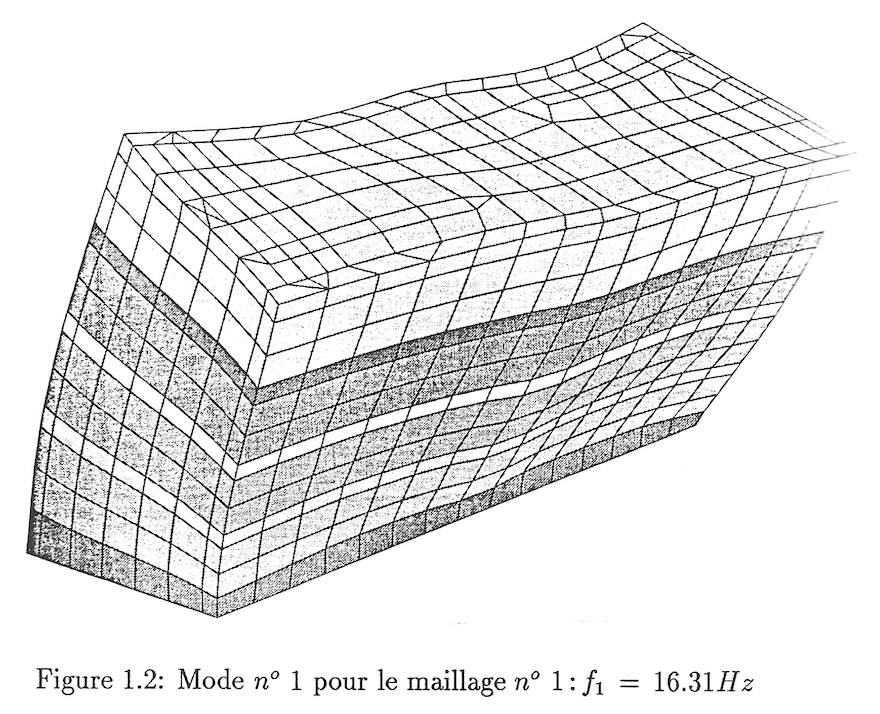
\includegraphics[scale=0.25]{castemLCPC01.png} 
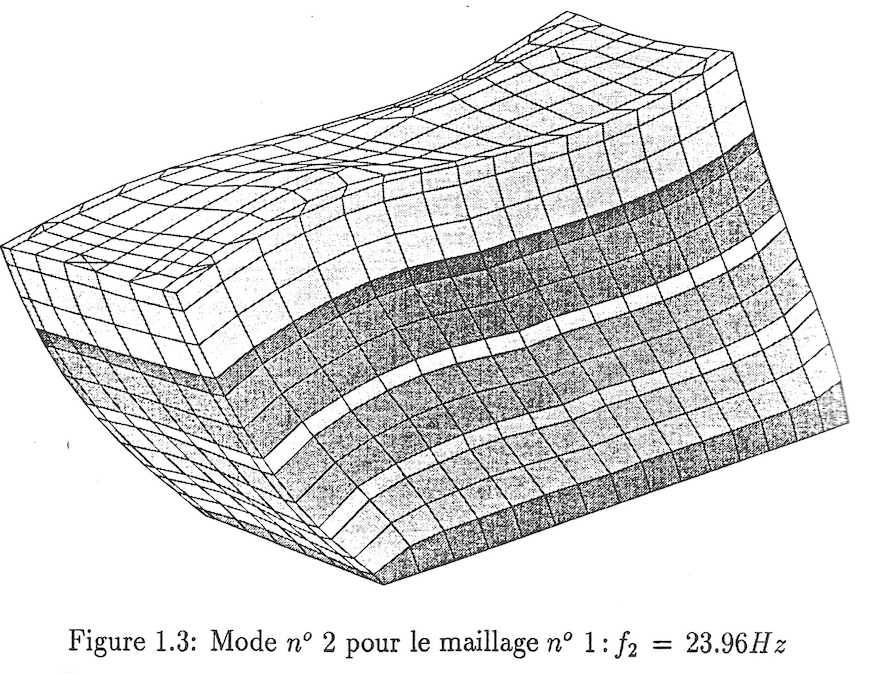
\includegraphics[scale=0.25]{castemLCPC02.png} 
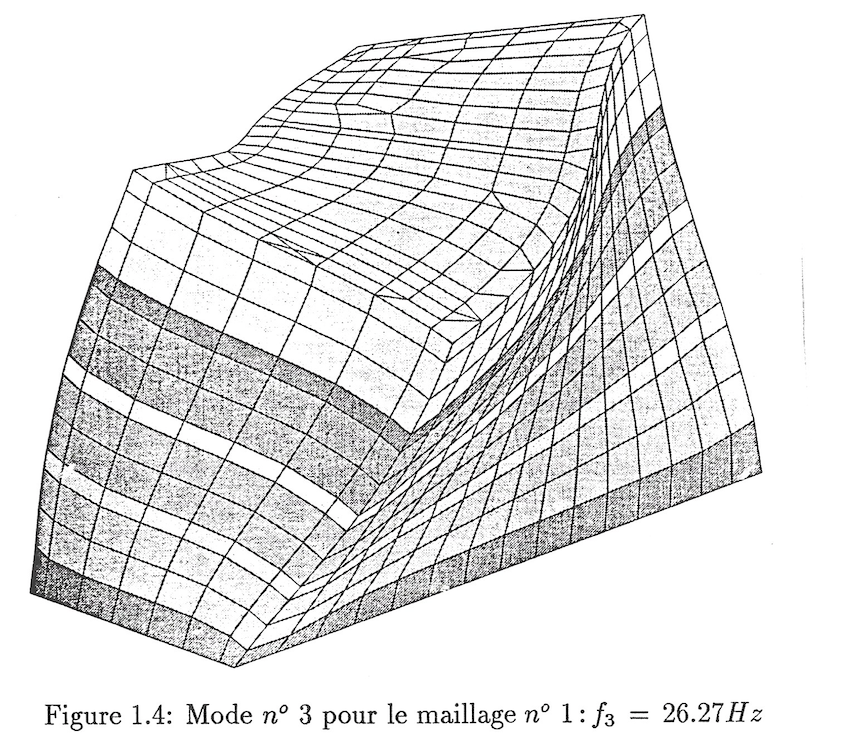
\includegraphics[scale=0.25]{castemLCPC03.png} 
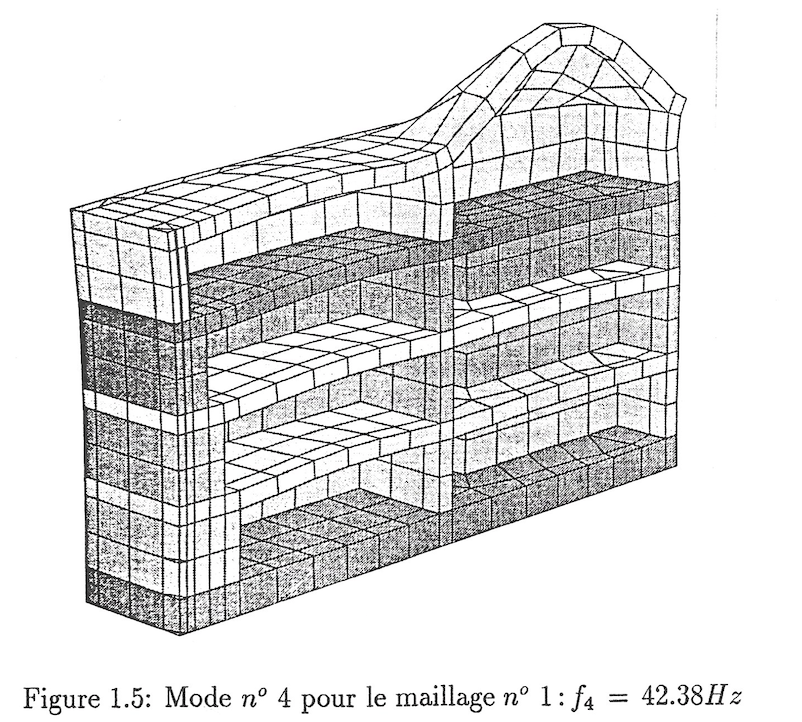
\includegraphics[scale=0.25]{castemLCPC04.png} 
\subsubsection*{Problèmes d'évolution}
\begin{itemize}[label=\textbullet, font=\small \color{blue}]
\item \underline{Problème parabolique:} 
\begin{enumerate}
\item équation de la chaleur, système de Stokes. 
\[\left\{\begin{array}{ll}
\frac{\partial u}{\partial t}-\Delta u = f &\mbox{dans }\; \Omega_T\\
u=0 &\mbox{sur }\; \Sigma_T\\
u(.,0)=u_0 &\mbox{dans }\; \Omega
\end{array}\right. \Longleftrightarrow \left\{\begin{array}{ll}
\mbox{ Trouver une fonction } u :&\\
u\in L^2(0,T;V)\cap {\cal C}^0(0,T;H), & \\
\frac{\de}{\de t}(u(t),v)+a(u(t),v)=(f(t),v) & \mbox{où } a(u,v)=\int_\Omega \nabla u\cdot \nabla v \; \de x\\
u(0)=u_0 &
\end{array}\right.\]
\item  Méthode de semi-discrétisation.
\[\forall v_h\in V_h \quad a(w_{i,h},v_h)=\lambda_{i,h} (w_{i,h},v_h)\]
\[u_h(t)=\sum_{i=1}^N\left\{(u_{0,h},w_{i,h})e^{-\lambda_{i,h}t}+\int_0^t(f(s),w_{i,h})e^{-\lambda_{i,h}(t-s)}\de s\right\}w_{i,h}\]
\item  Discrétisation totale.
\[\frac{1}{\Delta t}(y_{n+1}-y_n)=\theta\;\varphi(t_{n+1},y_{n+1})+(1-\theta)\;\varphi(t_{n},y_{n}),\quad 0\leq n\leq N-1\]
\end{enumerate}





\item \underline{Problème hyperbolique:} équation des ondes. Semi-discrétisation et discrétisation totale.

\begin{enumerate}
\item équation de la chaleur, système de Stokes. 
\[\left\{\begin{array}{ll}
\frac{\partial^2 u}{\partial t^2}-\Delta u = f &\mbox{dans }\; \Omega_T\\
u=0 &\mbox{sur }\; \Sigma_T\\
u(.,0)=u_0,\; \frac{\partial u}{\partial t} (.,0)=u_1&\mbox{dans }\; \Omega
\end{array}\right. \Longleftrightarrow \left\{\begin{array}{ll}
\mbox{ Trouver une fonction } u :&\\
u\in  {\cal C}^0(0,T;V)\cap {\cal C}^1(0,T;H), & \\
\frac{\de^2}{\de t^2}(u(t),v)+a(u(t),v)=(f(t),v) & \mbox{où } a(u,v)=\int_\Omega \nabla u\cdot \nabla v \; \de x\\
u(0)=u_0\; \frac{\partial u}{\partial t} (0)=u_1 &
\end{array}\right.\]
\item  Méthode de semi-discrétisation.
\[\forall v_h\in V_h \quad a(w_{i,h},v_h)=\lambda_{i,h} (w_{i,h},v_h)\]
On pose $\omega_{i,h}=\sqrt{\lambda_{i,h}}$
\[u_h(t)=\sum_{i=1}^N\left\{(u_{0,h},w_{i,h})\cos\omega_{i,h}t+\frac{1}{\omega_{i,h}}(u_{1,h},w_{i,h})\sin\omega_{i,h}t+\frac{1}{\omega_{i,h}}\int_0^t(f(s),w_{i,h})\sin(\omega_{i,h}(t-s))\de s\right\}w_{i,h}\]
\item  Discrétisation totale.
\[\left\{\begin{array}{l}
y_{n+1}=y_n+\Delta t z_n+\Delta t^2\left(\beta \varphi_{n+1}+\left(\frac 12-\beta\right)\varphi_n\right)\\
z_{n+1}=z_n+\Delta t (\gamma\;\varphi_{n+1}+(1-\gamma)\;\varphi_{n}),\quad 0\leq n\leq N-1
\end{array} \right.\]

\end{enumerate}


\end{itemize}
\subsection*{Exemples  avec CAST3M20}
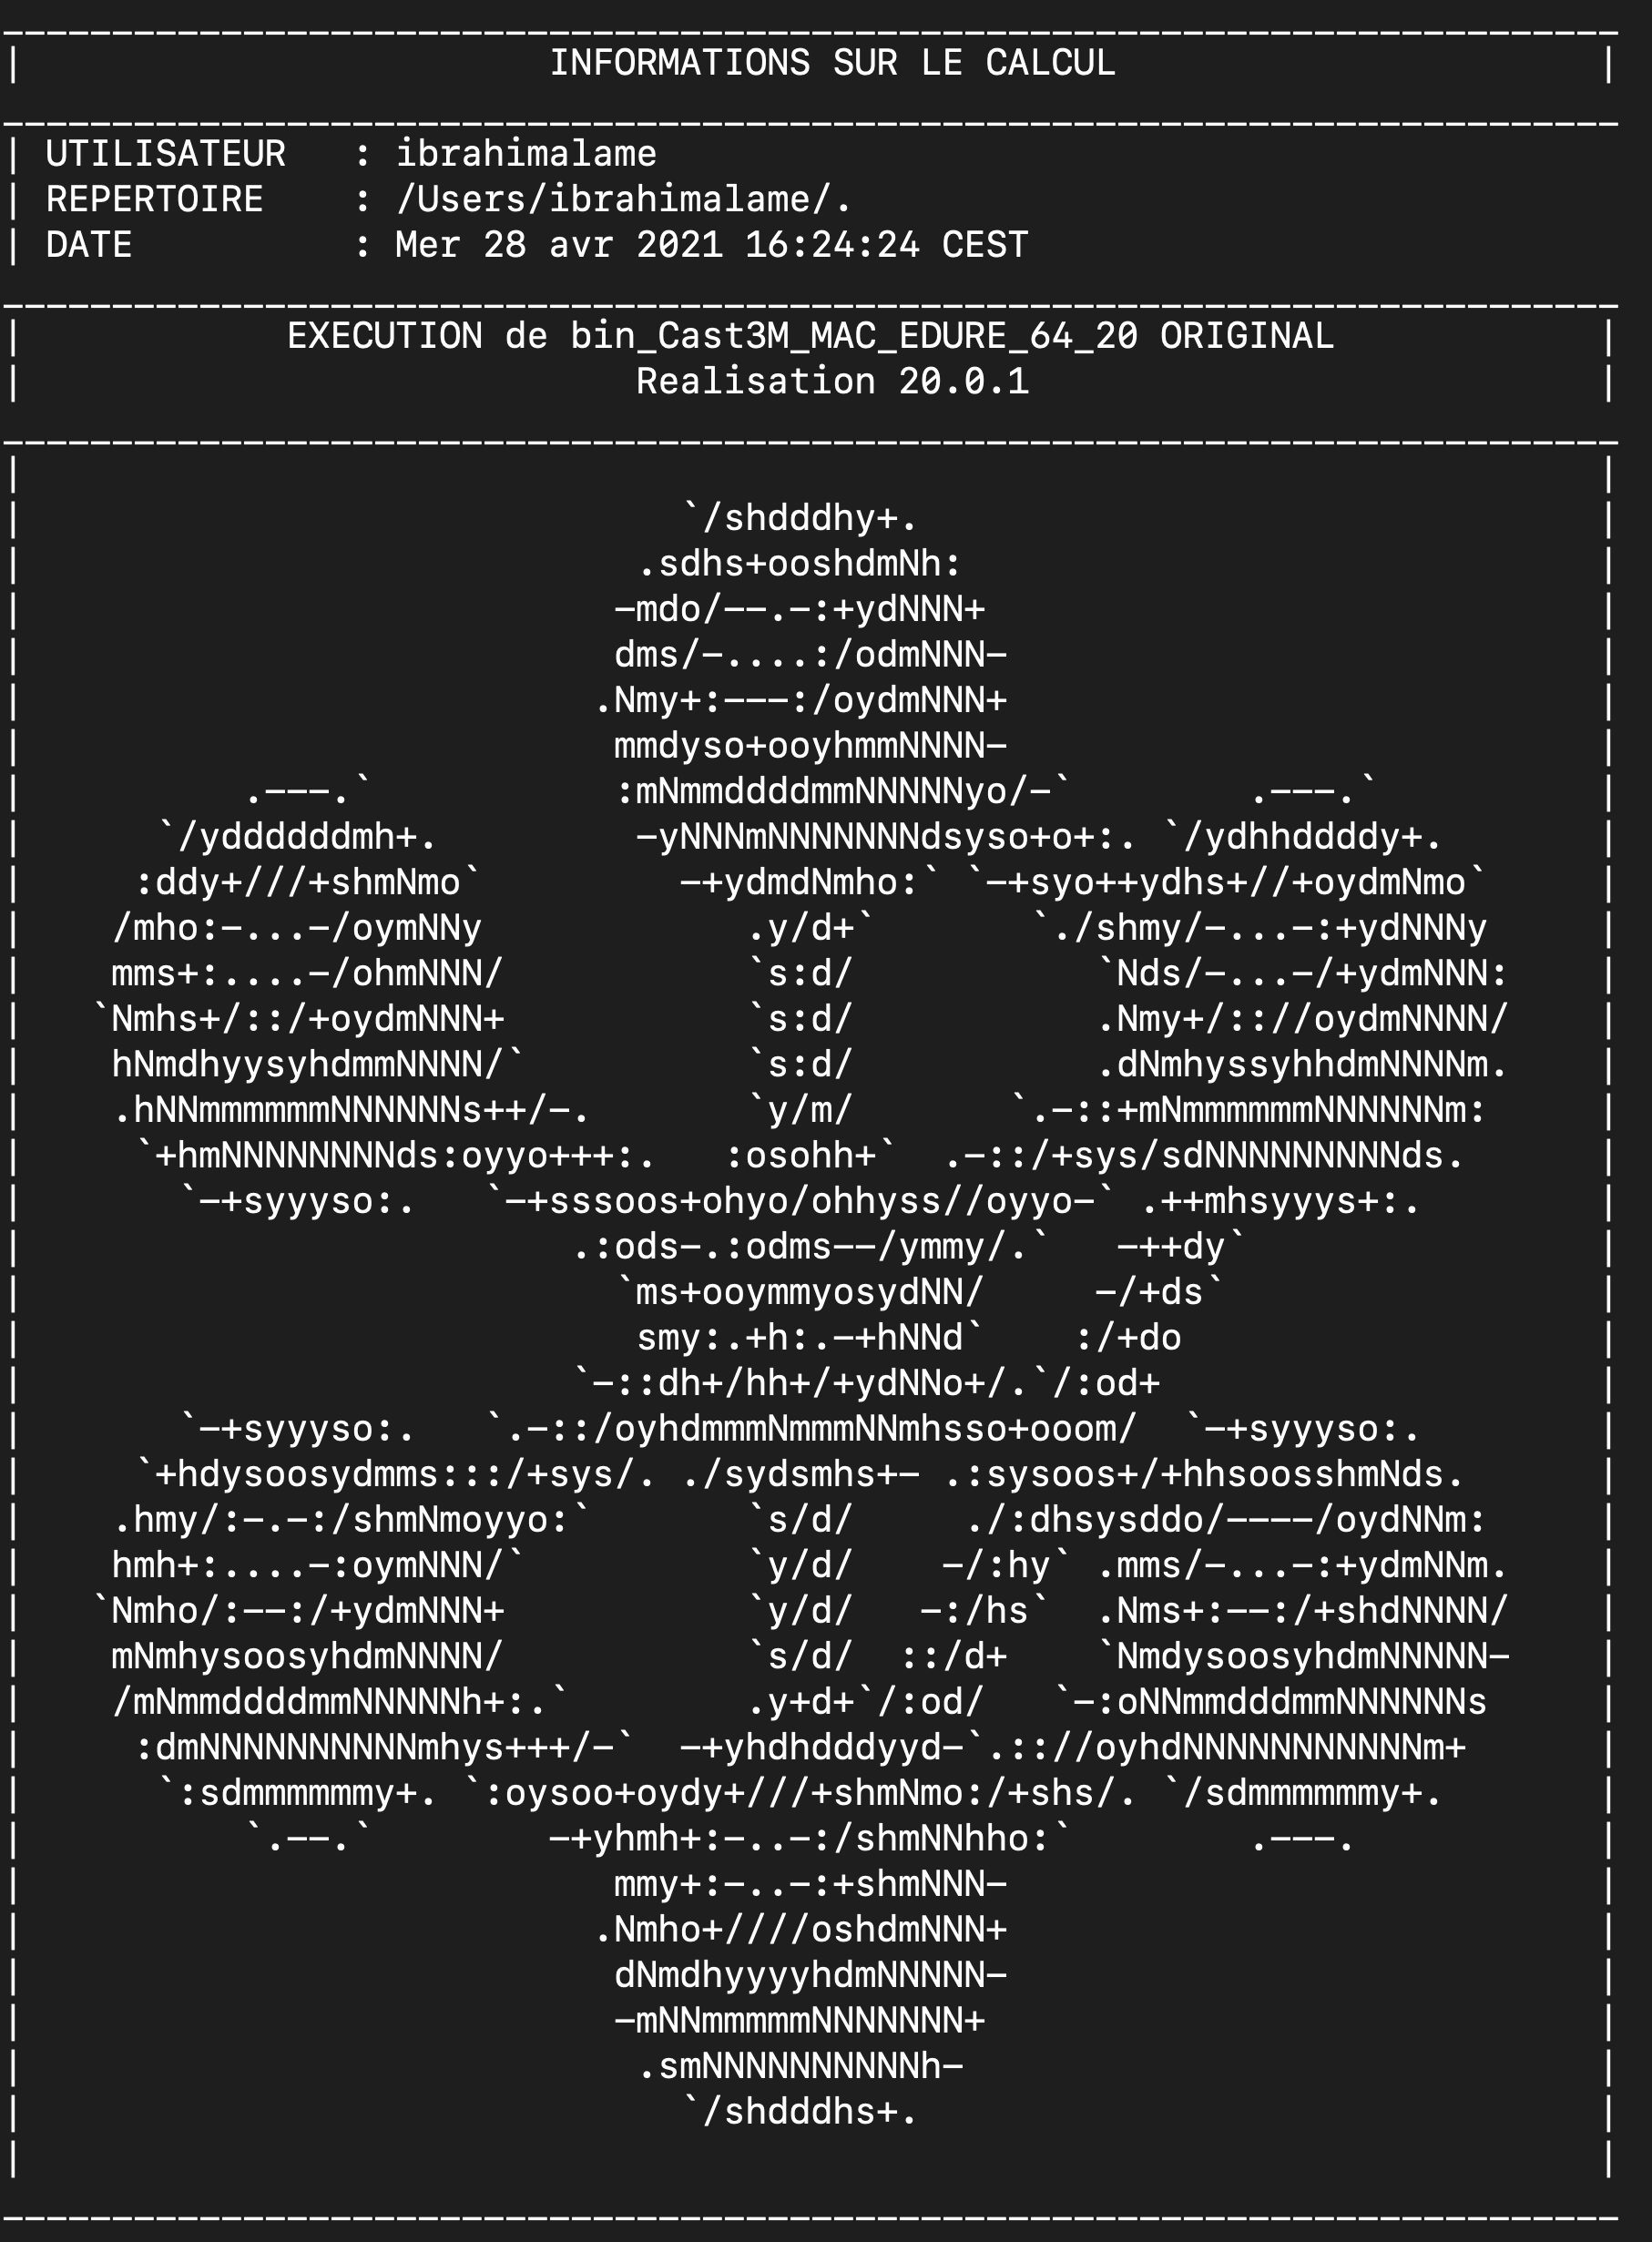
\includegraphics[scale=0.25]{castemVideo02.png} 
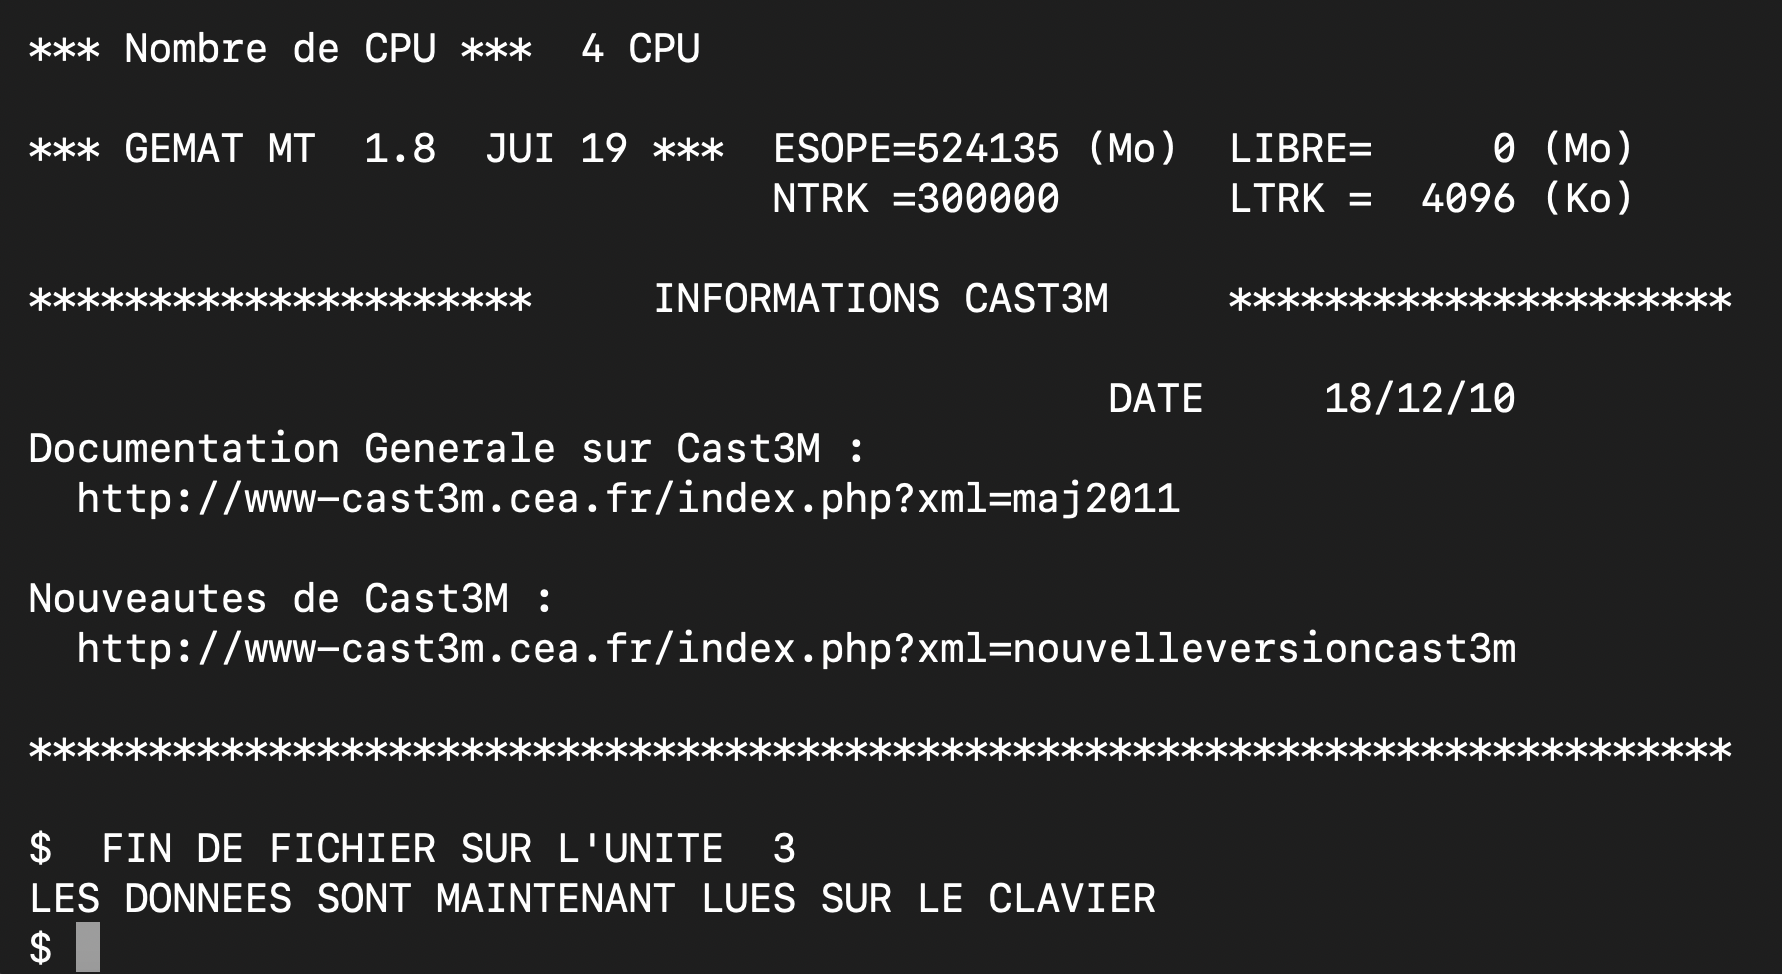
\includegraphics[scale=0.25]{castemVideo03.png} 
\begin{verbatim}

opti dime 3 elem cub8;
l1 = (0 0 0)droi (0 0.03 0) 3;
S1 = L1 tran (0 0 0.1) 10;
V1 = S1 volu tran (1. 0 0) 50;
trac V1 cach titr 'poutre' ;
mo1 = mode V1 mecanique elastique isotrope;
ma1 = mate mo1 youn 30.e9 nu 0.2;
trac ma1 mo1;

CL1 = bloq depl S1;

ptx1 = (V1 coor 1) point maxi;
trac ((ptx1 coul roug) et (aret V1));
F1=forc ptx1 (0 0 -1000);
trac (F1 vect forc vert)(aret V1);
k1 = rigi mo1 ma1;
k1= k1 et cl1;
u1 = reso k1 F1;
# Taille de la matrice: 997728 Facteur: 8.0591     Conditionnement: 0.0000     Performance #(Gflop/s): 1.7290
trac u1 V1;
def0 = defo u1 (aret V1) 0. blan ;
def1 = defo u1 V1 roug;
trac (def0 et def1);

\end{verbatim}

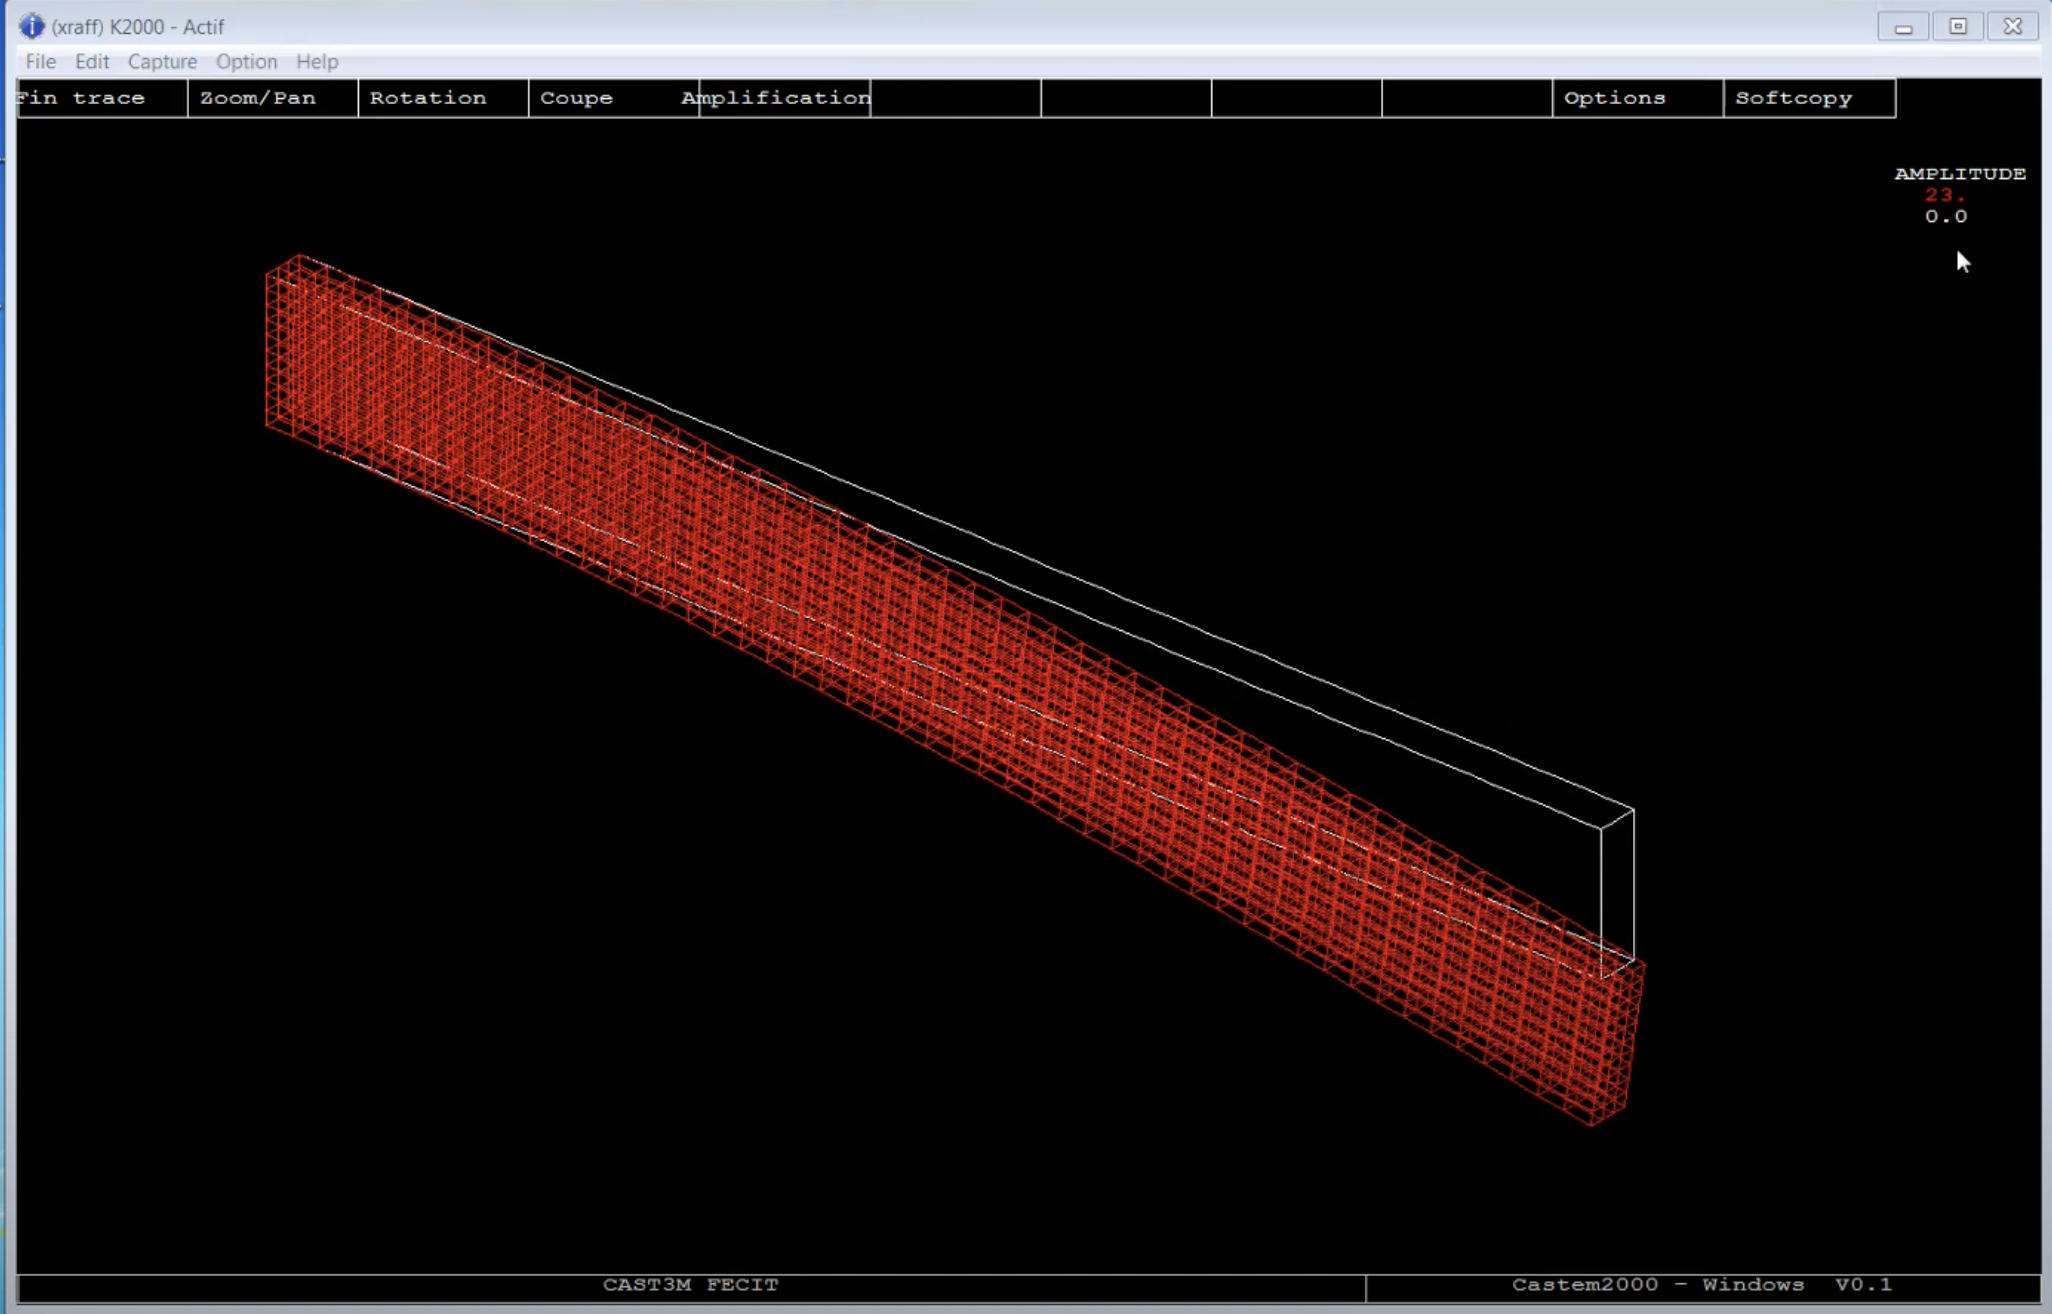
\includegraphics[scale=0.4]{castemVideo01.png} 



 \end{document}
 
opti dime 3 elem cub8;
l1 = (0 0 0)droi (0 0.03 0) 3;
S1 = L1 tran (0 0 0.1) 10;
V1 = S1 volu tran (1. 0 0) 50;
trac V1 cach titr 'poutre' ;
mo1 = mode V1 mecanique elastique isotrope;
ma1 = mate mo1 youn 30.e9 nu 0.2;
trac ma1 mo1;

CL1 = bloq depl S1;

ptx1 = (V1 coor 1) point maxi;
trac ((ptx1 coul roug) et (aret V1));
F1=forc ptx1 (0 0 -1000);
trac (F1 vect forc vert)(aret V1);
k1 = rigi mo1 ma1;
k1= k1 et cl1;
u1 = reso k1 F1;
# Taille de la matrice: 997728 Facteur: 8.0591     Conditionnement: 0.0000     Performance #(Gflop/s): 1.7290
trac u1 V1;
def0 = defo u1 (aret V1) 0. blan ;
def1 = defo u1 V1 roug;
trac (def0 et def1);


